\documentclass{article}

\usepackage{amsmath}
\usepackage{amssymb}
\usepackage{mathpartir}
\usepackage{fontawesome5}
\usepackage{xcolor}
\usepackage{tikz}
\mprset{flushleft}
\newcommand{\kw}[1]{\text{\textbf{#1}}}
\newcommand{\Let}[3]{\kw{let}\, #1 = #2\, \kw{in}\, #3}
\newcommand{\Fun}[2]{\kw{fun}\, #1 \Rightarrow #2}
\newcommand{\App}[2]{#1\, #2}
\newcommand{\Pair}[2]{(#1, #2)}
\newcommand{\LetPair}[4]{\kw{let}\, (#1, #2) = #3\, \kw{in}\, #4}
\newcommand{\Inl}[1]{\kw{left}(#1)}
\newcommand{\Inr}[1]{\kw{right}(#1)}
\newcommand{\Match}[5]{\kw{match}\, #1\, \kw{with}\, \Inl{#2} \Rightarrow #3 \mid \Inr{#4} \Rightarrow #5}
\newcommand{\AnnotSub}[1]{%
  \if\relax\detokenize{#1}\relax
  \else
    _{\smash{\raisebox{-0.25ex}{$\scriptstyle #1$}}}
  \fi}
\newcommand{\RefCell}[1]{\kw{ref}\, #1}
\newcommand{\Deref}[1]{\ !#1}
\newcommand{\Assign}[2]{#1 := #2}
\newcommand{\AnnotArrow}[1]{%
  \if\relax\detokenize{#1}\relax
    \to
  \else
    \xrightarrow[\AnnotBelow{#1}]{}
  \fi}
\newcommand{\AnnotBinop}[2]{%
  \if\relax\detokenize{#2}\relax
    #1
  \else
    \underset{\AnnotBelow{#2}}{#1}
  \fi}
\newcommand{\AnnotBelow}[1]{\smash{\raisebox{0.25ex}{$\scriptstyle #1$}}}
\newcommand{\TFun}[3][]{#2 \mathrel{\AnnotArrow{#1}} #3}
\newcommand{\TPair}[3][]{#2 \mathbin{\AnnotBinop{\times}{#1}} #3}
\newcommand{\TSum}[3][]{#2 \mathbin{\AnnotBinop{+}{#1}} #3}
\newcommand{\TRef}[2][]{\kw{ref}\AnnotSub{#1}\, #2}
\newcommand{\TUnit}{\kw{unit}}
\newcommand{\TEmpty}{\kw{empty}}
\newcommand{\UnitTerm}{\kw{unit}}
\newcommand{\Absurd}[1]{\kw{absurd}\, #1}
\newcommand{\judge}[3]{#1 \vdash #2 : #3}
\newcommand{\Jud}[2]{\judge{\Gamma}{#1}{#2}}
\newcommand{\leqto}{\mathrel{\leq_{\mathrm{to}}}}
\newcommand{\leqin}{\mathrel{\leq_{\mathrm{in}}}}
\newcommand{\mode}[1]{\textsc{#1}}
\newcommand{\subtype}{\mathrel{\sqsubseteq}}
\newcommand{\Sub}[2]{#1 \subtype #2}
\newcommand{\alias}{\mathrel{\underset{\AnnotBelow{\text{alias}}}{\rightsquigarrow}}}
\newcommand{\Alias}[2]{#1 \alias #2}
\newcommand{\Lock}[2][]{
  \text{\faLock}_{#1}(#2)
}
\newcommand{\ClampMap}[2]{%
  \begin{minipage}{0.23\linewidth}
    \centering
    \begin{tikzpicture}[scale=0.8]
      \foreach \x/\y in {#2} {
        \fill[blue!25] (\x,\y) rectangle ++(1,1);
      }
      \draw[very thick] (0,0) rectangle (4,4);
      \draw[step=1cm,gray!70] (0,0) grid (4,4);
      \foreach \v in {0,...,3} {
        \node[below] at (\v + 0.5,-0.12) {$\v$};
        \node[left] at (-0.12,\v + 0.5) {$\v$};
      }
    \end{tikzpicture}\\[2pt]
    \footnotesize #1
  \end{minipage}
}

\newcommand{\jules}[1]{{\textcolor{red}{\textbf{J}: #1}}}

\title{Borrowing Notes}
\author{Jules Jacobs}
\date{\today}

\begin{document}

\maketitle

\noindent
Extend areality with borrowing:
\begin{itemize}
    \item $0 = \mode{global}$
    \item $1 = \mode{regional}$
    \item $2 = \mode{local}$
    \item $3 = \mode{borrowed}$
\end{itemize}
where $0 \leq 1 \leq 2 \leq 3$, i.e. $\mode{global} \leq \mode{regional} \leq \mode{local} \leq \mode{borrowed}$.

\paragraph{Global modality}
The global modality maps all points to $\mode{global}$, except for $\mode{borrowed}$ which is mapped to itself.

\begin{align*}
    f(x) = \begin{cases}
        0 & \text{if } x \in \{0,1,2\} \\
        3 & \text{if } x = 3 \\
    \end{cases}
\end{align*}


It has the following left adjoint:

\begin{align*}
    g(x) = \begin{cases}
        0 & \text{if } x = 0 \\
        3 & \text{if } x \in \{1,2,3\} \\
    \end{cases}
\end{align*}

It has the following right adjoint:

\begin{align*}
    h(x) = \begin{cases}
        2 & \text{if } x \in \{0,1,2\} \\
        3 & \text{if } x = 3 \\
    \end{cases}
\end{align*}

Pictorially:

\begin{center}
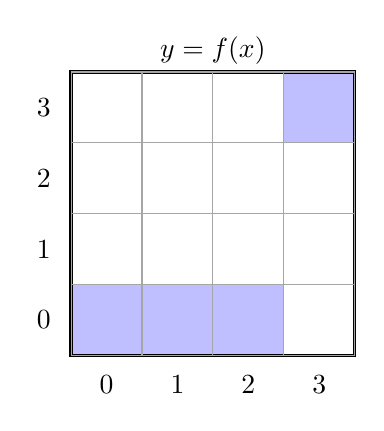
\begin{tikzpicture}[scale=0.9]
  \foreach \x/\y in {0/0,1/0,2/0,3/3} {
    \fill[blue!25] (\x,\y) rectangle ++(1,1);
  }
  \draw[very thick] (0,0) rectangle (4,4);
  \draw[step=1cm,gray!70] (0,0) grid (4,4);
  \foreach \v in {0,...,3} {
  \node[below] at (\v + 0.5,-0.15) {$\v$};
  \node[left] at (-0.15,\v + 0.5) {$\v$};
}
  \node at (2,4.3) {$y = f(x)$};
\end{tikzpicture}
\end{center}

\medskip

Because the lattice only has four elements, we can witness each adjunction by shading the pairs that satisfy the defining inequalities. Blue cells highlight the points where the inequality is tight, making the graphs of \(f\), \(g\), and \(h\) easy to spot.

\paragraph{Left adjoint $g \dashv f$}
The condition \(g(y) \leq x \iff y \leq f(x)\) means both relations pick out exactly the same lattice points:

\begin{center}
\begin{minipage}{0.45\linewidth}
\centering
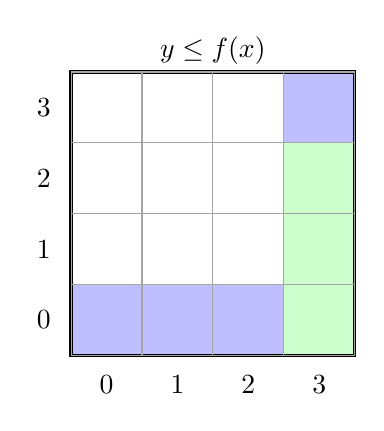
\begin{tikzpicture}[scale=0.9]
  \foreach \x in {0,...,2} {
    \fill[green!20] (\x,0) rectangle ++(1,1);
  }
  \foreach \y in {0,...,3} {
    \fill[green!20] (3,\y) rectangle ++(1,1);
  }
  \foreach \x/\y in {0/0,1/0,2/0,3/3} {
    \fill[blue!25] (\x,\y) rectangle ++(1,1);
  }
  \draw[very thick] (0,0) rectangle (4,4);
  \draw[step=1cm,gray!70] (0,0) grid (4,4);
  \foreach \v in {0,...,3} {
    \node[below] at (\v + 0.5,-0.15) {$\v$};
    \node[left] at (-0.15,\v + 0.5) {$\v$};
  }
  \node at (2,4.3) {$y \leq f(x)$};
\end{tikzpicture}
\end{minipage}\hfill
\begin{minipage}{0.45\linewidth}
\centering
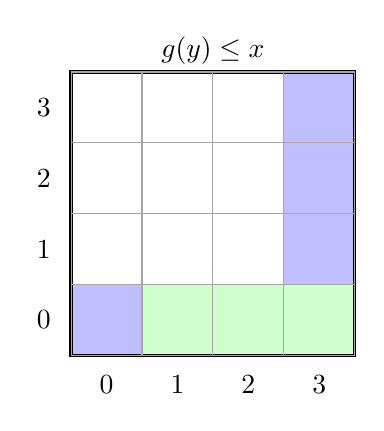
\begin{tikzpicture}[scale=0.9]
  \foreach \x in {0,...,3} {
    \fill[green!20] (\x,0) rectangle ++(1,1);
  }
  \foreach \y in {1,...,3} {
    \fill[green!20] (3,\y) rectangle ++(1,1);
  }
  \foreach \x/\y in {0/0,3/1,3/2,3/3} {
    \fill[blue!25] (\x,\y) rectangle ++(1,1);
  }
  \draw[very thick] (0,0) rectangle (4,4);
  \draw[step=1cm,gray!70] (0,0) grid (4,4);
  \foreach \v in {0,...,3} {
    \node[below] at (\v + 0.5,-0.15) {$\v$};
    \node[left] at (-0.15,\v + 0.5) {$\v$};
  }
  \node at (2,4.3) {$g(y) \leq x$};
\end{tikzpicture}
\end{minipage}
\end{center}

\smallskip
\noindent\emph{Slogan: the points below \(f\) (left) are exactly the points to the right of \(g\) (right).}

\medskip

\paragraph{Right adjoint $f \dashv h$}
Likewise, the right adjoint \(h\) is characterised by \(f(x) \leq y \iff x \leq h(y)\):

\begin{center}
\begin{minipage}{0.45\linewidth}
\centering
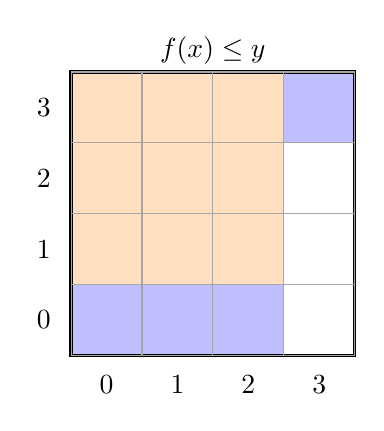
\begin{tikzpicture}[scale=0.9]
  \foreach \x in {0,...,2} {
    \foreach \y in {0,...,3} {
      \fill[orange!25] (\x,\y) rectangle ++(1,1);
    }
  }
  \fill[orange!25] (3,3) rectangle ++(1,1);
  \foreach \x/\y in {0/0,1/0,2/0,3/3} {
    \fill[blue!25] (\x,\y) rectangle ++(1,1);
  }
  \draw[very thick] (0,0) rectangle (4,4);
  \draw[step=1cm,gray!70] (0,0) grid (4,4);
  \foreach \v in {0,...,3} {
    \node[below] at (\v + 0.5,-0.15) {$\v$};
    \node[left] at (-0.15,\v + 0.5) {$\v$};
  }
  \node at (2,4.3) {$f(x) \leq y$};
\end{tikzpicture}
\end{minipage}\hfill
\begin{minipage}{0.45\linewidth}
\centering
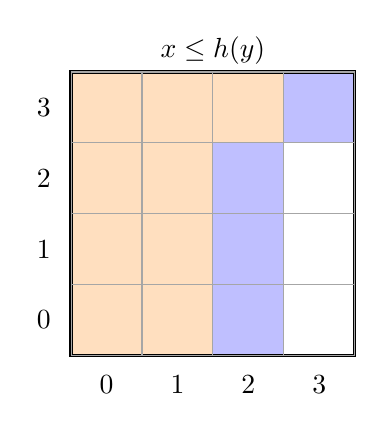
\begin{tikzpicture}[scale=0.9]
  \foreach \y in {0,...,2} {
    \foreach \x in {0,...,2} {
      \fill[orange!25] (\x,\y) rectangle ++(1,1);
    }
  }
  \foreach \x in {0,...,3} {
    \fill[orange!25] (\x,3) rectangle ++(1,1);
  }
  \foreach \x/\y in {2/0,2/1,2/2,3/3} {
    \fill[blue!25] (\x,\y) rectangle ++(1,1);
  }
  \draw[very thick] (0,0) rectangle (4,4);
  \draw[step=1cm,gray!70] (0,0) grid (4,4);
  \foreach \v in {0,...,3} {
    \node[below] at (\v + 0.5,-0.15) {$\v$};
    \node[left] at (-0.15,\v + 0.5) {$\v$};
  }
  \node at (2,4.3) {$x \leq h(y)$};
\end{tikzpicture}
\end{minipage}
\end{center}

\smallskip
\noindent\emph{Slogan: the points above \(f\) (left) are exactly the points to the left of \(h\) (right).}

\medskip

\paragraph{Clamping upward: $f_c(x) = \max(x,c)$}
For any constant \(c \in \{0,1,2,3\}\) consider the inflationary map \(f_c(x) = \max(x,c)\).  It always has a left adjoint
\[
g_c(y) =
\begin{cases}
0 & \text{if } y \leq c,\\
y & \text{if } y > c,
\end{cases}
\]
reflecting that any point below \(c\) ``backs off'' to the global mode while elements above \(c\) stay fixed.  When \(c = 0\) the map is the identity, so both adjoints coincide with \(f_c\).  For every \(c > 0\) there is \emph{no} right adjoint: if \(y < c\) then no element \(x\) satisfies \(\max(x,c) \leq y\), so the defining implication for a right adjoint would fail.

\paragraph{Clamping downward: $f_c(x) = \min(x,c)$}
Dually, the deflationary map \(f_c(x) = \min(x,c)\) always has a right adjoint
\[
h_c(y) =
\begin{cases}
y & \text{if } y < c,\\
3 & \text{if } y \geq c,
\end{cases}
\]
which keeps points strictly below \(c\) unchanged and collapses everything above \(c\) to the top mode \(3\).  This map has a left adjoint only in the trivial case \(c = 3\) (again the identity), because for any \(c < 3\) and \(y > c\) there is no \(x\) with \(y \leq \min(x,c)\).

\paragraph{Adjoint pictures (example $c = 2$)}
The adjunction laws become especially tangible on our four-point lattice.  Below we spell out the non-trivial clamp \(\max(x,2)\) together with its left adjoint \(g_2\), and \(\min(x,2)\) together with its right adjoint \(h_2\).

\begin{center}
\begin{minipage}{0.45\linewidth}
\centering
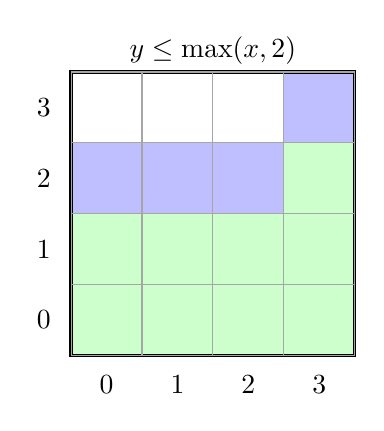
\begin{tikzpicture}[scale=0.9]
  \foreach \x in {0,...,2} {
    \foreach \y in {0,...,2} {
      \fill[green!20] (\x,\y) rectangle ++(1,1);
    }
  }
  \foreach \y in {0,...,3} {
    \fill[green!20] (3,\y) rectangle ++(1,1);
  }
  \foreach \x/\y in {0/2,1/2,2/2,3/3} {
    \fill[blue!25] (\x,\y) rectangle ++(1,1);
  }
  \draw[very thick] (0,0) rectangle (4,4);
  \draw[step=1cm,gray!70] (0,0) grid (4,4);
  \foreach \v in {0,...,3} {
    \node[below] at (\v + 0.5,-0.15) {$\v$};
    \node[left] at (-0.15,\v + 0.5) {$\v$};
  }
  \node at (2,4.3) {$y \leq \max(x,2)$};
\end{tikzpicture}
\end{minipage}\hfill
\begin{minipage}{0.45\linewidth}
\centering
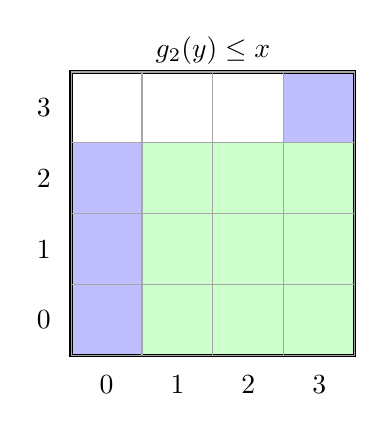
\begin{tikzpicture}[scale=0.9]
  \foreach \y in {0,...,2} {
    \foreach \x in {0,...,3} {
      \fill[green!20] (\x,\y) rectangle ++(1,1);
    }
  }
  \fill[green!20] (3,3) rectangle ++(1,1);
  \foreach \x/\y in {0/0,0/1,0/2,3/3} {
    \fill[blue!25] (\x,\y) rectangle ++(1,1);
  }
  \draw[very thick] (0,0) rectangle (4,4);
  \draw[step=1cm,gray!70] (0,0) grid (4,4);
  \foreach \v in {0,...,3} {
    \node[below] at (\v + 0.5,-0.15) {$\v$};
    \node[left] at (-0.15,\v + 0.5) {$\v$};
  }
  \node at (2,4.3) {$g_2(y) \leq x$};
\end{tikzpicture}
\end{minipage}
\end{center}

\smallskip
\noindent\emph{Slogan: the points below \(\max(x,2)\) (left) are exactly the points to the right of \(g_2\) (right).}

\medskip

\begin{center}
\begin{minipage}{0.45\linewidth}
\centering
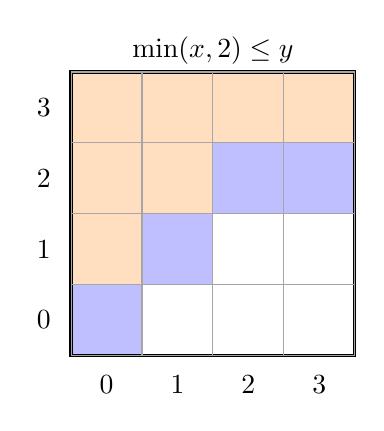
\begin{tikzpicture}[scale=0.9]
  \foreach \y in {0,...,3} {
    \fill[orange!25] (0,\y) rectangle ++(1,1);
  }
  \foreach \y in {1,...,3} {
    \fill[orange!25] (1,\y) rectangle ++(1,1);
  }
  \foreach \y in {2,...,3} {
    \fill[orange!25] (2,\y) rectangle ++(1,1);
    \fill[orange!25] (3,\y) rectangle ++(1,1);
  }
  \foreach \x/\y in {0/0,1/1,2/2,3/2} {
    \fill[blue!25] (\x,\y) rectangle ++(1,1);
  }
  \draw[very thick] (0,0) rectangle (4,4);
  \draw[step=1cm,gray!70] (0,0) grid (4,4);
  \foreach \v in {0,...,3} {
    \node[below] at (\v + 0.5,-0.15) {$\v$};
    \node[left] at (-0.15,\v + 0.5) {$\v$};
  }
  \node at (2,4.3) {$\min(x,2) \leq y$};
\end{tikzpicture}
\end{minipage}\hfill
\begin{minipage}{0.45\linewidth}
\centering
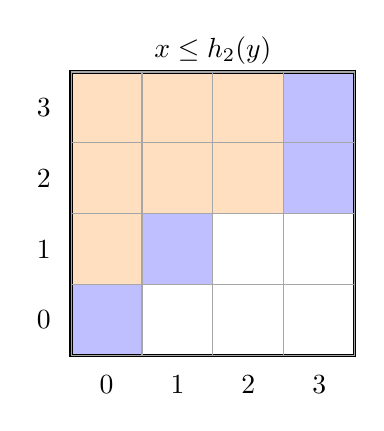
\begin{tikzpicture}[scale=0.9]
  \fill[orange!25] (0,0) rectangle ++(1,1);
  \foreach \x in {0,1} {
    \fill[orange!25] (\x,1) rectangle ++(1,1);
  }
  \foreach \x in {0,...,3} {
    \fill[orange!25] (\x,2) rectangle ++(1,1);
    \fill[orange!25] (\x,3) rectangle ++(1,1);
  }
  \foreach \x/\y in {0/0,1/1,3/2,3/3} {
    \fill[blue!25] (\x,\y) rectangle ++(1,1);
  }
  \draw[very thick] (0,0) rectangle (4,4);
  \draw[step=1cm,gray!70] (0,0) grid (4,4);
  \foreach \v in {0,...,3} {
    \node[below] at (\v + 0.5,-0.15) {$\v$};
    \node[left] at (-0.15,\v + 0.5) {$\v$};
  }
  \node at (2,4.3) {$x \leq h_2(y)$};
\end{tikzpicture}
\end{minipage}
\end{center}

\smallskip
\noindent\emph{Slogan: the points above \(\min(x,2)\) (left) are exactly the points to the left of \(h_2\) (right).}

\medskip

\noindent\textbf{Pictures.} The following grids show \(y = f_c(x)\) for every clamp level.  Blue squares highlight the equality points, just like in the earlier adjoint figures.

\begin{center}
\ClampMap{$\max(x,0)$}{0/0,1/1,2/2,3/3}\hspace{1em}
\ClampMap{$\max(x,1)$}{0/1,1/1,2/2,3/3}\hspace{1em}
\ClampMap{$\max(x,2)$}{0/2,1/2,2/2,3/3}\hspace{1em}
\ClampMap{$\max(x,3)$}{0/3,1/3,2/3,3/3}
\end{center}

\smallskip
\noindent\emph{Left to right: increasing the lower bound pushes more points upward while the left adjoint collapses the shaded columns back to $0$ or fixes them.}

\medskip

\begin{center}
\ClampMap{$\min(x,0)$}{0/0,1/0,2/0,3/0}\hspace{1em}
\ClampMap{$\min(x,1)$}{0/0,1/1,2/1,3/1}\hspace{1em}
\ClampMap{$\min(x,2)$}{0/0,1/1,2/2,3/2}\hspace{1em}
\ClampMap{$\min(x,3)$}{0/0,1/1,2/2,3/3}
\end{center}

\smallskip
\noindent\emph{Left to right: lowering the ceiling flattens more of the graph, and the right adjoint \(h_c\) matches the columns where the clamp leaves inputs unchanged.}

\end{document}
